\documentclass[11pt,a4paper]{article}
\usepackage[utf8]{inputenc}
\usepackage{amsmath,amsfonts,amssymb}
\usepackage{graphicx}
\usepackage{geometry}
\geometry{margin=1in}
\usepackage{booktabs}
\usepackage{hyperref}
\usepackage{float}
\usepackage{xcolor}

\title{\textbf{EE3621: Digital Signal Processing} \\ \Large Lecture 23: Digital Oscillators, Waveform Generation \& NCO \\ \large (III B.Tech EEE)}
\author{Lecture Notes (40-Minute Plan)}
\date{}

\definecolor{darkbg}{HTML}{0d121f}
\definecolor{lighttext}{HTML}{e2e8f0}
\definecolor{primary}{HTML}{8b5cf6}
\definecolor{secondary}{HTML}{0dd5c5}

\pagecolor{darkbg}
\color{lighttext}

\hypersetup{
    colorlinks=true,
    linkcolor=secondary,
    urlcolor=secondary
}

\begin{document}

\maketitle

\section{Lecture Plan \& Objectives (40 Minutes Breakdown)}
\begin{itemize}
    \item \textbf{00:00 -- 05:00 (5 mins):} Need for Digital Oscillators in DSP (SDR, modems).
    \item \textbf{05:00 -- 15:00 (10 mins):} Recursive Oscillator (IIR approach), derivations, and coupled equations.
    \item \textbf{15:00 -- 20:00 (5 mins):} Poles on the unit circle, stability issues, amplitude drift.
    \item \textbf{20:00 -- 25:00 (5 mins):} Amplitude correction methods (Rotor method).
    \item \textbf{25:00 -- 32:00 (7 mins):} Numerically Controlled Oscillator (NCO) and DDS. Phase noise and spurs.
    \item \textbf{32:00 -- 35:00 (3 mins):} Chirp signal generation (LFM).
    \item \textbf{35:00 -- 40:00 (5 mins):} Checkpoint Questions and Summary.
\end{itemize}

\noindent\rule{\textwidth}{0.5pt}

\section{Need for Digital Oscillators}

\begin{figure}[H]
    \centering
    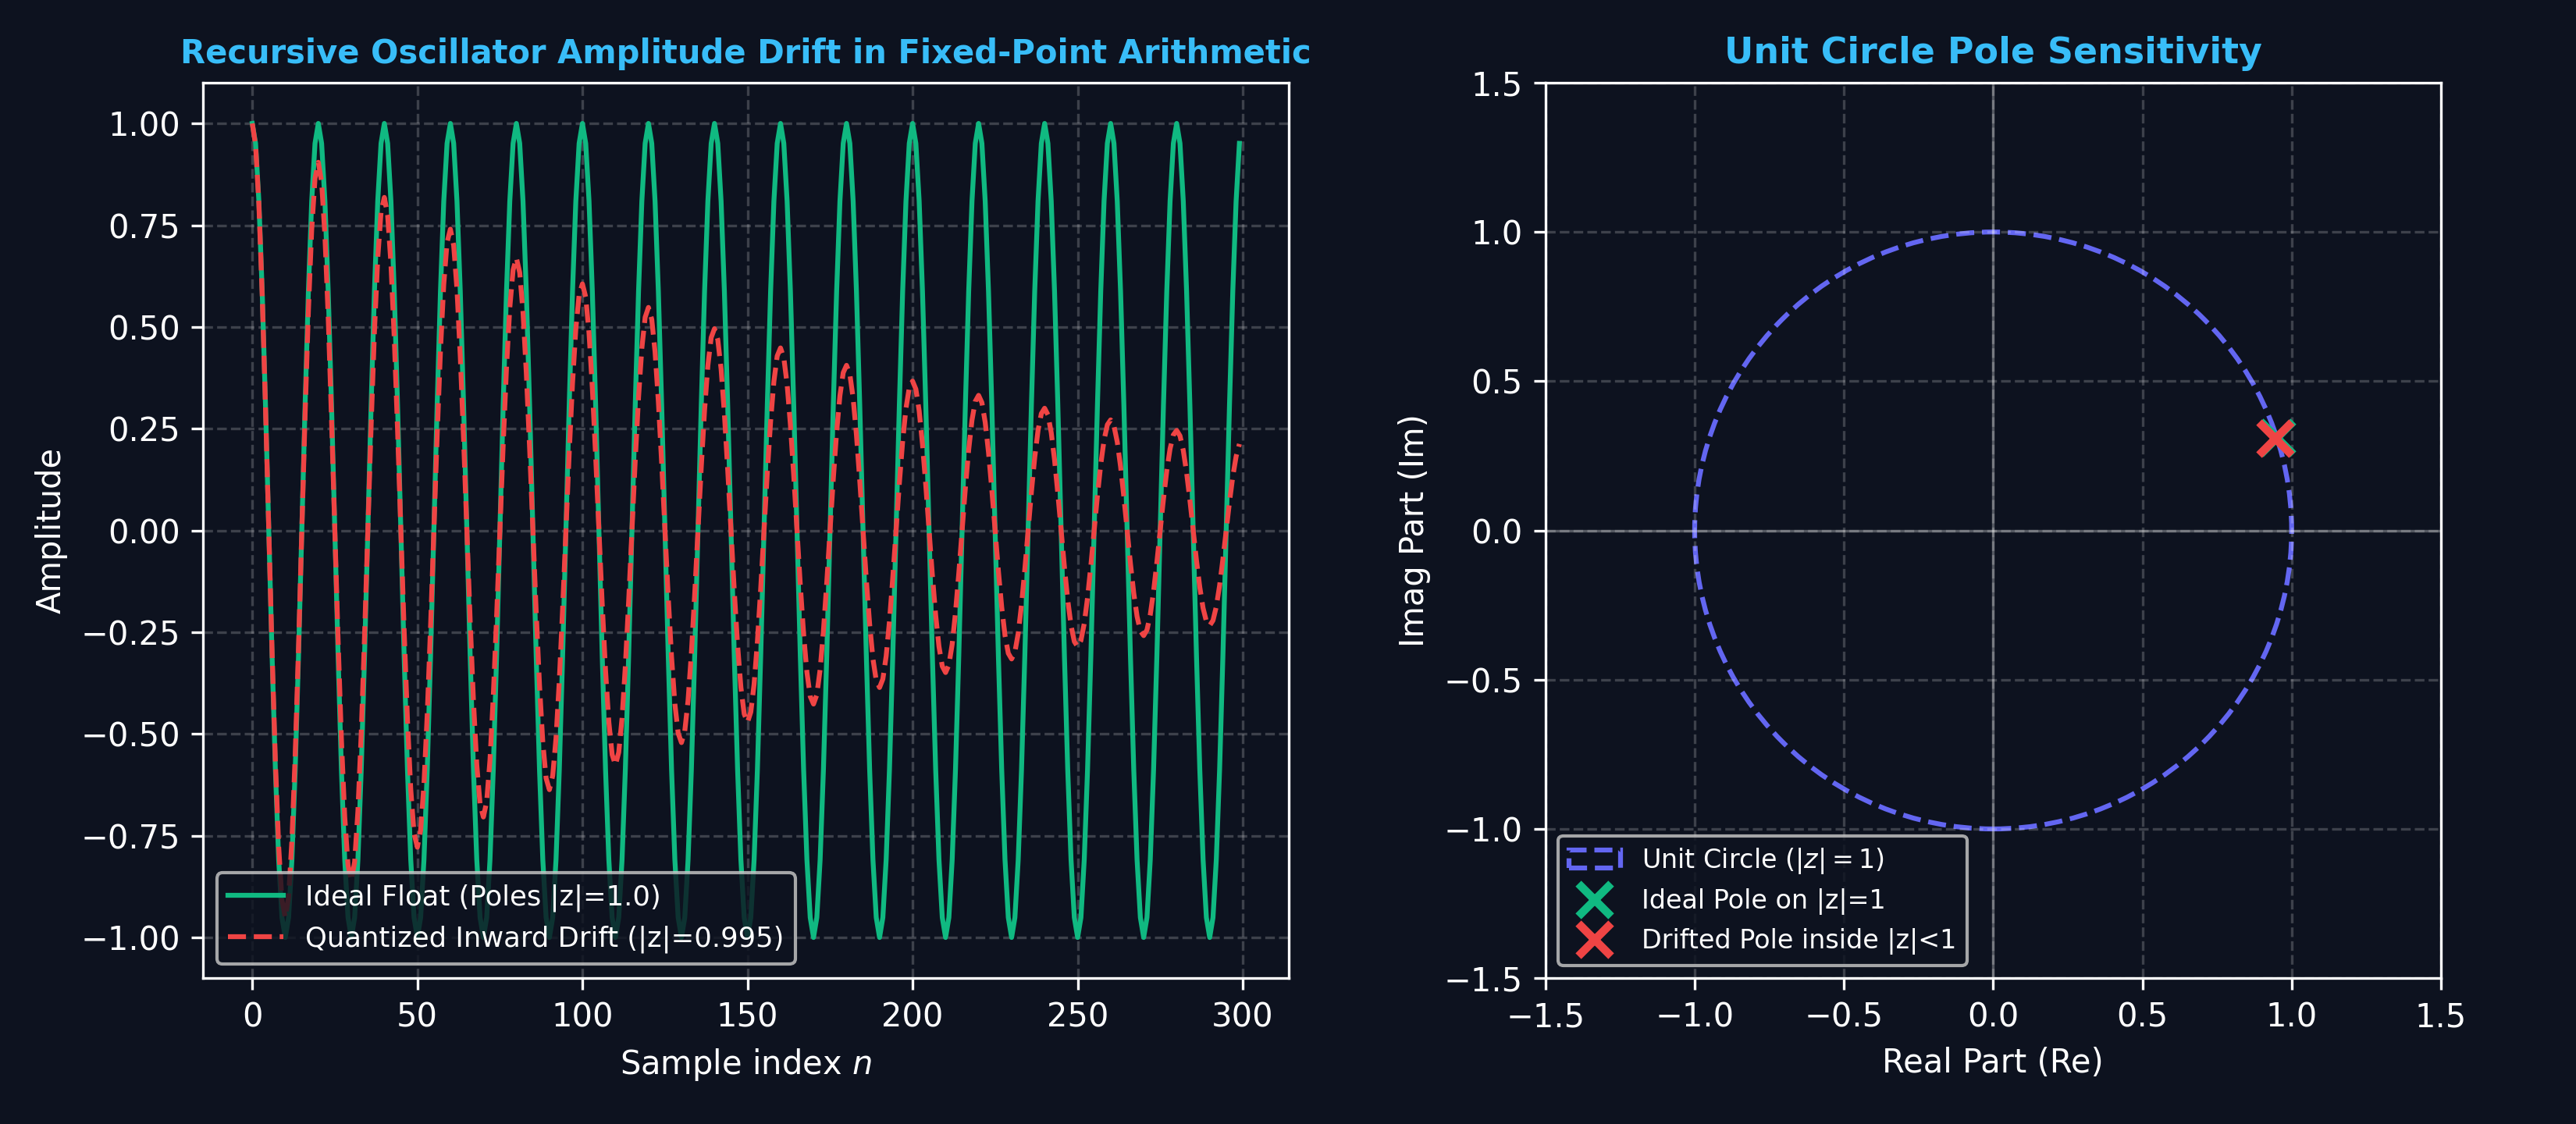
\includegraphics[width=0.85\textwidth]{images/recursive_oscillator_zplane_drift.png}
    \caption{Fixed-Point Coefficient Sensitivity: Unit-Circle Pole Quantization Drift and Amplitude Instability.}
\end{figure}

\begin{figure}[H]
    \centering
    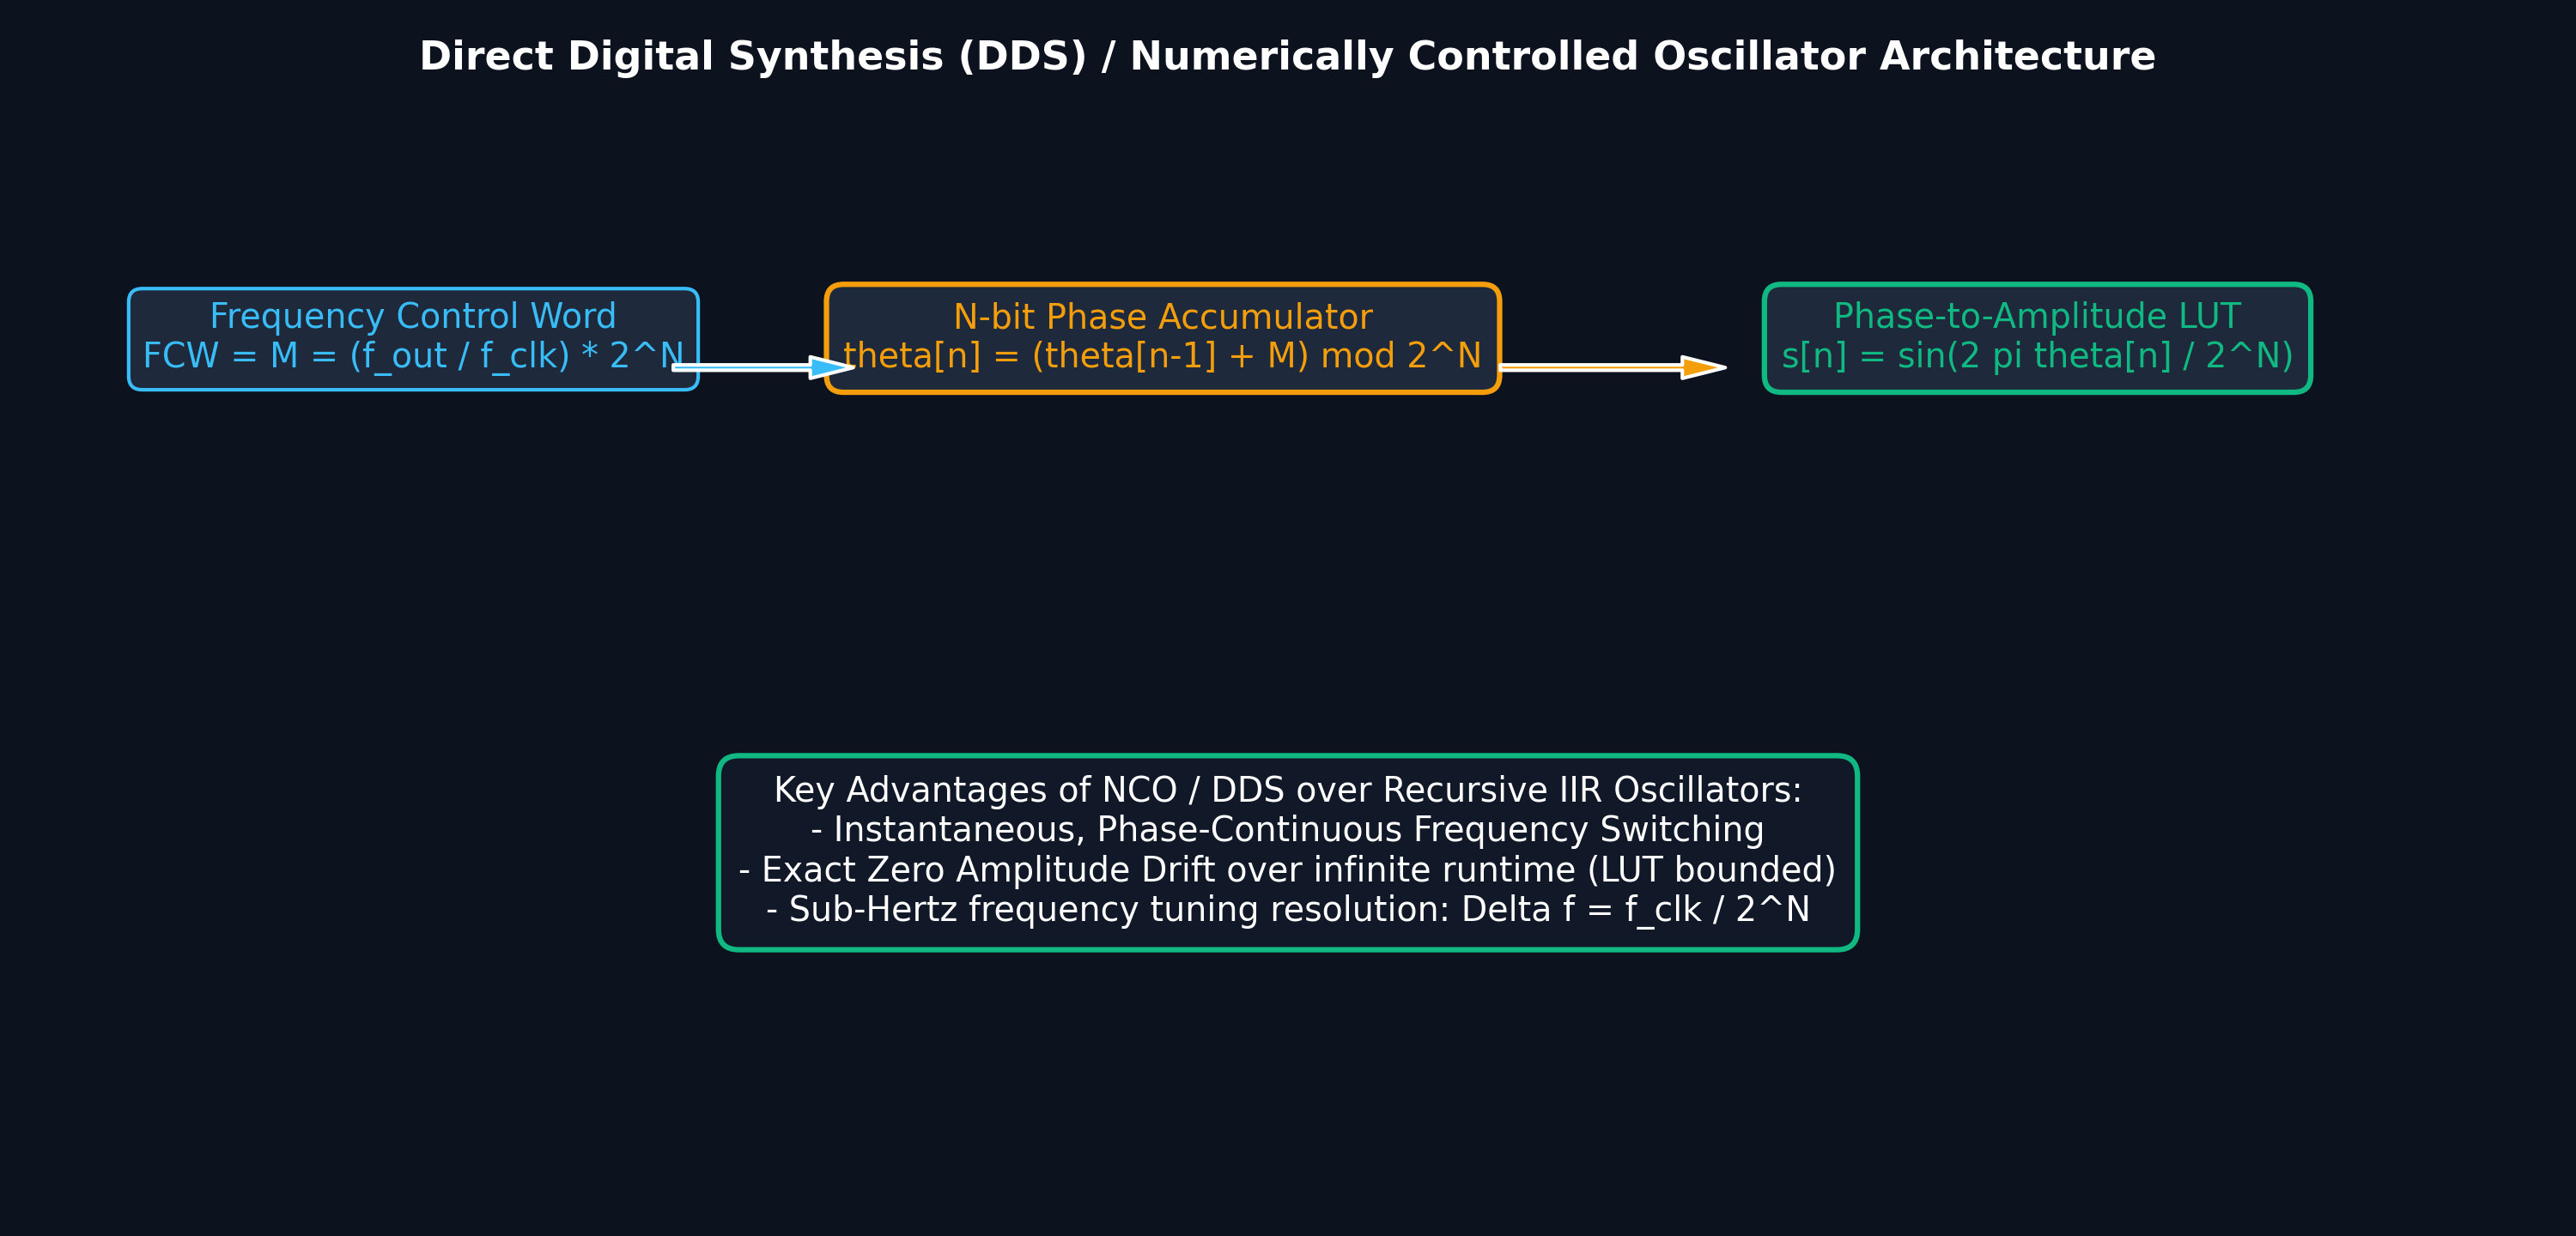
\includegraphics[width=0.85\textwidth]{images/dds_nco_architecture_operation.png}
    \caption{Direct Digital Synthesis (DDS / NCO) Architecture: Phase Accumulator and Sine Look-Up Table (LUT).}
\end{figure}


In modern digital systems, generating precise waveforms entirely in the digital domain is crucial. Digital oscillators replace bulky and temperature-sensitive analog Voltage-Controlled Oscillators (VCOs) with digital equivalents. 

Applications include Software-Defined Radio (SDR) for digital up/down-conversion, Modems for carrier generation, and arbitrary waveform generation for test equipment. They offer exact reproducibility without thermal drift.

\section{Recursive Oscillator (IIR Approach)}
We can generate a sinusoid by realizing a discrete-time system whose impulse response is a sinusoid.
Consider the complex exponential sequence:
\begin{equation}
y[n] = e^{j\omega_0 n}
\end{equation}

\textbf{Derivation of the difference equation:}
\begin{enumerate}
    \item Sum of exponentials at adjacent times $n+1$ and $n-1$: 
    \begin{equation*}
    y[n+1] + y[n-1] = e^{j\omega_0 (n+1)} + e^{j\omega_0 (n-1)}
    \end{equation*}
    \item Factor out $e^{j\omega_0 n}$: 
    \begin{equation*}
    y[n+1] + y[n-1] = e^{j\omega_0 n} (e^{j\omega_0} + e^{-j\omega_0})
    \end{equation*}
    \item Apply Euler's identity $e^{j\omega_0} + e^{-j\omega_0} = 2\cos(\omega_0)$:
    \begin{equation*}
    y[n+1] + y[n-1] = 2\cos(\omega_0) y[n]
    \end{equation*}
    \item Shift time index by $-1$:
    \begin{equation}
    y[n] = 2\cos(\omega_0) y[n-1] - y[n-2]
    \end{equation}
\end{enumerate}

To generate both sine and cosine without direct-form stability issues, we separate real and imaginary parts for coupled oscillator equations:
\begin{align}
c[n] &= 2\cos(\omega_0)c[n-1] - c[n-2] \\
s[n] &= 2\cos(\omega_0)s[n-1] - s[n-2]
\end{align}
This only needs a multiplier and two unit delays per channel.

\section{Poles on the Unit Circle and Amplitude Drift}
Taking the Z-transform of the oscillator difference equation:
\begin{equation}
H(z) = \frac{z^{-1}}{1 - 2\cos(\omega_0)z^{-1} + z^{-2}}
\end{equation}
The roots of the denominator are strictly on the unit circle: $z = e^{\pm j\omega_0}$.
Because the poles are precisely on the unit circle, the system is marginally stable. In fixed-point arithmetic, coefficient quantization and round-off noise cause the amplitude to drift exponentially (decay or grow).

\section{Amplitude Correction}
To combat drift, periodic normalization can be used, scaling states by the inverse of instantaneous amplitude. 
Alternatively, the Rotor method implements complex multiplication directly:
\begin{equation}
y[n] = e^{j\omega_0} y[n-1]
\end{equation}
requiring only 4 real multiplies and 2 adds per sample.

\section{Numerically Controlled Oscillator (NCO) \& DDS}
An NCO explicitly tracks phase and maps it to amplitude via a Lookup Table (LUT). 
At each clock $f_s$, we add the phase increment $\Delta\phi$:
\begin{equation}
\Phi = (\Phi + \Delta\phi) \pmod{2^B}
\end{equation}
\begin{equation}
f_{out} = \frac{\Delta\phi \cdot f_s}{2^B}
\end{equation}
Direct Digital Synthesis (DDS) combines an NCO with a DAC and LPF. 
\textbf{Phase Truncation \& Spurs:} Because LUT addresses are truncated, predictable spurious tones appear at $f_{spur} = k\cdot f_s/2^B$. Dithering (adding random noise before truncation) is used to randomize these spurs and improve Spurious-Free Dynamic Range (SFDR).

\section{Chirp Signal Generation}
Linear frequency modulation (LFM):
\begin{equation}
x[n] = \cos\left(\omega_0 n + \frac{\mu}{2}n^2\right)
\end{equation}
Generated by feeding an NCO with a linearly increasing tuning word. Applications include RADAR and sonar.

\section{Illustrative Plots}
For signal envelope bounding and spur suppression visualization, window functions are often applied:

\section{Checkpoints}
\textbf{Q1: Why does a recursive digital oscillator suffer from amplitude drift?} \\
\textit{Answer:} Poles must be precisely on the unit circle. Fixed-point coefficient quantization moves them off the circle, causing exponential growth or decay. Accumulated roundoff noise also contributes.

\textbf{Q2: NCO with 32-bit accumulator, 100 MHz clock. Tuning word for 1 MHz?} \\
\textit{Answer:} $f_{out} = (\Delta\phi \cdot f_s)/2^B \implies \Delta\phi = (10^6 \cdot 2^{32})/10^8 \approx 42949673$.

\textbf{Q3: Why dither an NCO phase?} \\
\textit{Answer:} It randomizes periodic phase truncation errors, spreading spur energy into the noise floor and improving SFDR.

\section{Key Formulas}
\begin{table}[H]
\centering
\begin{tabular}{@{}ll@{}}
\toprule
\textbf{Concept} & \textbf{Formula} \\ \midrule
Recursive Oscillator & $y[n] = 2\cos(\omega_0)y[n-1] - y[n-2]$ \\
Coupled Form & $c[n] = 2\cos(\omega_0)c[n-1] - c[n-2]$ \\
Transfer Function & $H(z) = \frac{z^{-1}}{1 - 2\cos(\omega_0)z^{-1} + z^{-2}}$ \\
NCO Output Freq & $f_{out} = \frac{\Delta\phi \cdot f_s}{2^B}$ \\
Chirp Phase & $\phi[n] = \omega_0 n + \frac{\mu}{2}n^2$ \\ \bottomrule
\end{tabular}
\end{table}

\end{document}
